% !TeX root = ../main.tex

\chapter{面向分布式架构的高效算法设计}


\section{概述}\label{sec:dist-overview}
% 怎么拓展到Billion-Scale?现有方法怎么做的?


\section{方法介绍}\label{sec:dist-method}

\subsection{混合并行分布式算法建模}\label{sec:dist-method-model}
% 本章节的并行是针对机器的,例如是多机之间?单机内部?

\subsection{索引预先加载策略}\label{sec:dist-method-index}
% 命中率越来越高,近存那部分工作可以放在这里
最后,我们提出了预取邻居列表策略来隐藏查找和过滤操作的时间开销。为了便于描述,这里不考虑延迟排序队列策略。在原始的搜索算法计算流程中,$i$ -th步骤的距离计算操作依赖于$i$ -th步骤的邻居列表,这使得查找&过滤操作无法与其他操作并行。这里我们首先定义\textit{潜在的未搜索点}($p_{pu}$),它是队列中最小的$Dist.$和$Flag$为真的点(除了最近的未搜索点)。我们发现$(i-1)$ -th步骤的潜在未搜索点有很大的概率成为$i$ -th步骤的搜索点(我们称之为搜索命中)。为了进一步量化这一现象,我们将$n$ -th步骤中的搜索命中率定义为$(n+l)$ -th步骤。
\begin{equation}\label{eq:hit rate}
hit\ rate = \frac{1}{l}\sum\limits_{i=n+1}\limits^{n+l}{\left| p_s^{(i)} = p_{pu}^{(i-1)} \right|}
\end{equation}

如图\ref{fig:hit rate}所示,我们将搜索过程平均分成十个部分,然后分别计算每个部分的搜索命中率。实验结果表明,除前20\%的步骤外,其余80\%的步骤的平均搜索命中率为82.6\% ~ 84.1\%。也就是说,我们可以根据$(i-1)$ -th步骤的潜在未搜索点提前执行Lookup&Filter操作,以便$i$ -th步骤的距离计算操作不必等待$i$ -th步骤的Lookup&Filter操作(如果它命中)。
我们需要添加一个更改来实现这个策略。在选择操作中,我们首先确定搜索是否命中。如果没有被命中,我们需要根据搜索点重新执行查找和过滤操作。

\begin{figure}
  \centering
  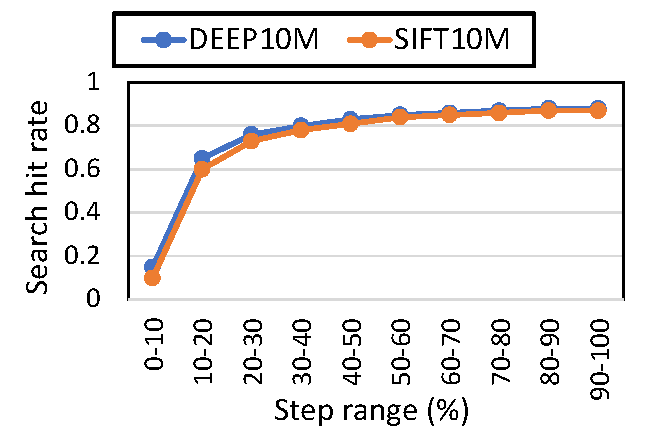
\includegraphics[width=0.5\textwidth]{figures/context-2/hitrate.pdf}
  \caption{The search hit rate varies with the search step (R@10 is 0.97). The average hit rate of the last 80\% steps is 82.6\%-84.1\%.}
  \label{fig:hitrate}
\end{figure}

\subsection{特征延迟处理策略}\label{sec:dist-method-feature}



\section{实验结果}\label{sec:dist-experiment}
\subsection{实验设置}

\subsection{实现方法}
% 在FPGA上进行了验证

\subsection{整体性能}

\subsection{消融实验}



\section{本章小结}\label{sec:dist-conclusion}